\section{L3}


\subsection{Perfect secrecy II}

\subparagraph{Formal definition of perfect secrecy (\textbf{Definition 2})}

For every \(m, m' \in \M\) and every \(c \in \C\),
\[\Pr[\Enc_K(m) = c] = \Pr[\Enc_K(m') = c]\]

\subparagraph{Example: shift cipher}

\(\Pr[M = \letter{a}] = 0.7\) \\
\(\Pr[M = \letter{z}] = 0.3\)

Let \(m = \letter{a}\), and \(m' = \letter{z}\). \\
Then
\[ \Pr[\Enc_K(\letter{a}) = \letter{b}] = \frac{1}{26} =
\Pr[\Enc_K(\letter{z}) = \letter{b}] \]

(For further explanantion, if \(\Enc_K(\letter{a}) = \letter{b}\), \(K\) must be \(1\), where probability is \(\frac{1}{26}\); similarly, if \(\Enc_K(\letter{z}) = \letter{b}\), \(K\) must be \(2\). That's why their probabilities are same.)

\subparagraph{Lemma}

An encryption scheme \(\Pi = (\Gen, \Enc, \Dec)\) with message space is perfectly secret (which means \(\Pi\) satisfies Def. 1), the above equation (which is Def. 2) holds for every \(m, m' \in \M\) and every \(c \in \C\).

意即 Def. 1 等價 (equivalent) 於 Def. 2.

\pagebreak

\subparagraph{Proof of Def. 2 to Def. 1}

Fix a \(\dist(\M)\), a message \(m\) and a ciphertext \(c\) for which \(\Pr[C = c] > 0\). \\
If \(\Pr[M = m] = 0\), then \(\Pr[M = m \mid C = c] = \Pr[M = m]\). It always holds. \\
If \(\Pr[M = m] > 0\):
\begin{myEnumerate}[label=(\roman*)]
	\item \( \Pr[C = c \mid M = m] = \Pr[\Enc_K(M) = c \mid M = m] = \Pr[\Enc_K(m) = c] = \mathbf{\alpha} \)
	
	\item For every \(m' \in \M\),
	\[ \Pr[C = c \mid M = m'] = \Pr[\Enc_K(M) = c \mid M = m'] = \Pr[\Enc_K(m') = c] = \mathbf{\alpha} \]
	
	\item By Bayes' Theorem, 
	\begingroup
	\addtolength{\jot}{1em}
	\begin{align*}
		\Pr[M = m \mid C = c]
				&= \frac{\Pr[C = c \mid M = m] \cdot \Pr[M = m]}{\Pr[C = c]} \\
				&= \frac{\Pr[C = c \mid M = m] \cdot \Pr[M = m]}{\sum_{m' \in \M} \Pr[C = c \mid M = m'] \cdot \Pr[M = m']} \tag{by (i) and (ii)}\\
				& = \frac{\alpha \cdot \Pr[M = m]}{\sum_{m' \in \M} \ \alpha \cdot \Pr[M = m']} \\
				& = \frac{\alpha \cdot \Pr[M = m]}{\alpha \cdot \sum_{m' \in \M} \ \Pr[M = m']} \\
				& = \frac{\cancel\alpha \cdot \Pr[M = m]}{\cancel\alpha \cdot \sum_{m' \in \M} \ \Pr[M = m']} \\
				& = \Pr[M = m]
	\end{align*}
	\endgroup
\end{myEnumerate}

\pagebreak

\subparagraph{Proof of Def. 1 to Def. 2 (Quiz)}

Fix a \(\dist(\M)\), a message \(m\) and a ciphertext \(c\) for which \(\Pr[C = c] > 0\). \\
If \(\Pr[C = c] = 0\), then \(\Pr[C = c \mid M = m] = \Pr[C = c \mid M = m'] = 0\). It always holds. \\
If \(\Pr[C = c] > 0\): \\
(i) For \(\Pr[\Enc_K(m) = c]\),
\begin{align*}
	\Pr[\Enc_K(m) = c] &= Pr[C = c \mid M = m]\\
	&= \frac{\Pr[M = m \mid C = c] \cdot \Pr[C = c]}{\Pr[M = m]} \\
	&= \frac{\Pr[M = m] \cdot \Pr[C =c]}{\Pr[M = m]} \tag{by Def. 1}\\
	&= \frac{\cancel{\Pr[M = m]} \cdot \Pr[C = c]}{\cancel{\Pr[M = m]}} \\
	&= \Pr[C = c]
\end{align*}

(ii) For \(\Pr[\Enc_K(m') = c]\),
\begin{align*}
	\Pr[\Enc_K(m) = c] &= Pr[C = c \mid M = m']\\
	&= \frac{\Pr[M = m' \mid C = c] \cdot \Pr[C = c]}{\Pr[M = m']} \\
	&= \frac{\Pr[M = m'] \cdot \Pr[C =c]}{\Pr[M = m']} \tag{by Def. 1} \\
	&= \frac{\cancel{\Pr[M = m']} \cdot \Pr[C = c]}{\cancel{\Pr[M = m']}} \\
	&= \Pr[C = c]
\end{align*}

From (i) and (ii), we know that
\[ \Pr[\Enc_K(m) = c] = \Pr[\Enc_K(m') = c] \]


\subsection{Perfect secrecy III}

\subparagraph{Adversarial indistinguishability}

Adversarial indistinguishable experiment
\[PrivK_{A, \Pi}^{eav}\]
其中 \(A\) 代表 adversary, \(\Pi\) 代表 scheme, and \(eav\) 代表 eavesdropper.

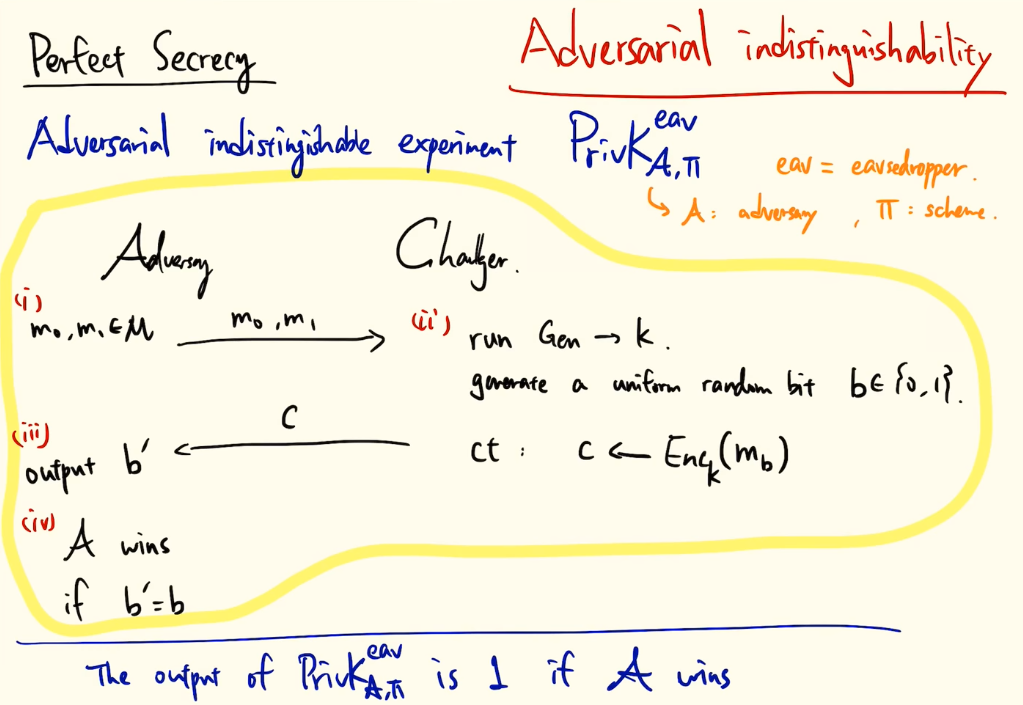
\includegraphics[width=0.8\textwidth, keepaspectratio]{adversarial_indistinguishability.png}

這個 experiment 有兩個人:adversary 和 Challenger。
\begin{steps}
	\item Adversary 會從 message space 中選出兩份訊息 \(m_0\) 和 \(m_1\),並這兩份訊息發送給 Challenger。
	\item Challenger 會執行 key generation algorithm \(Gen\) 來產生 key \(k\),並 generate 一個 uniform random bit \(b \in \{0,1\}\)。最後產生出 ciphertext \(c \leftarrow \Enc_k(m_b)\),再將 \(c\) 回傳給 adversary。
	\item Adversary 會 output 一個 \(b'\) 來代表它猜測 \(b\) 的結果。
	\item 若 \(b' = b\),則 adversary 成功猜對了。
\end{steps}

這個 experiment \(PrivK_{A, \Pi}^{eav}\) 的 output 就是 adversary 是否猜對;也可以說,當 \(PrivK_{A, \Pi}^{eav} = 1\),則 \(b' = b\)。


\subparagraph{Formal definition of perfect secrecy (\textbf{Definition 3, defined by perfect indistinguishability})}

\(\Pi = (\Gen, \Enc, \Dec)\) with message space \(\M\) is perfectly indistinguishable if for every adversary \(A\), it holds
\[\Pr[PrivK_{A, \Pi}^{eav} = 1] = \frac{1}{2}\]

意思:猜中的機率為 \(\frac{1}{2}\),和沒有 \(c\) 的前提下,隨便亂猜的機率(即 \(\Pr[(\text{randomly output} \ b' ) \wedge (b' = b)] = \frac{1}{2}\))是一樣的。代表 \(c\) 並沒有洩漏任何額外資訊。

這個命題和 \(\Pr[PrivK_{A, \Pi}^{eav} = 0] = \frac{1}{2}\) 是等價的。

注意:若 \(\Pr[PrivK_{A, \Pi}^{eav} = 1] < \frac{1}{2}\) 並不代表攻擊者更不會猜。因為 \(\Pr[PrivK_{A, \Pi}^{eav} = 1] + \Pr[PrivK_{A, \Pi}^{eav} = 0] = 1\),所以 \(\Pr[PrivK_{A, \Pi}^{eav} = 0] > \frac{1}{2}\)。因此猜另一種情況的正確機率會更高。

\subparagraph{Lemma}

\(\Pi\) is perfectly secret if and only if it is perfectly indistinguishable.

\subparagraph{Proof of Def. 2 to Def. 3}

由 Def. 2 可知
\[
	\Pr[\Enc_K(m_0) = c] = \Pr[\Enc_K(m_1) = c]
\]

又因為 \(c \leftarrow \Enc_k(m_b)\),所以
\begin{align*}
	\Pr[\Enc_K(m_0) = c] = \Pr[b = 0] \\
	\Pr[\Enc_K(m_1) = c] = \Pr[b = 1]
\end{align*}

因此 \(\Pr[b = 0] = \Pr[b = 1] = \displaystyle\frac{1}{2}\)(因為在本例中 \(\Pr[b = 0] + \Pr[b = 1] = 1\))。

\begin{align*}
	\Pr[PrivK_{A, \Pi}^{eav}] &= \Pr[b' = b] \\
	&= \Pr[b' = b \wedge b = 0] + \Pr[b' = b \wedge b = 1] \tag{rewrite} \\
	&= \Pr[b' = b \mid b = 0] \times \Pr[b = 0] + \Pr[b' = b \mid b = 1] \times \Pr[b = 1] \tag{rewrite} \\
	&= \Pr[b' = 0]  \times \Pr[b = 0] + \Pr[b' = 1] \times \Pr[b = 1] \tag{rewrite} \\
	&= \Pr[b' = 0]  \times \frac{1}{2} + \Pr[b' = 1] \times \frac{1}{2} \tag{by Def. 2 denoted above} \\
	&= \frac{1}{2}(\Pr[b' = 0] + \Pr[b' = 1]) \\
	&= \frac{1}{2}	\tag{\(\because \Pr[b' = 0] + \Pr[b' = 1] = 1\)}
\end{align*}

\subparagraph{Proof of Def. 3 to Def. 2 (Bonus)}

%TODO


\subsection{One-Time Pad (OTP)}

\subparagraph{Construction of OTP}

Fix an integer \(l\) > 0, and let \(|\M| = |\C| = |\K| = l\). \\
(whch means all are binary strings of length \(l\), i.e., \(\{0, 1\}^l\))

Key generation algorithm \(\Gen\): uniformly randomly chooses a key \(k \in \K\), \(k\) is \(l\)-bit key.

Encryption algorithm \(\Enc\): given \(k \in \{0, 1\}^l\) and a message \(m \in \{0, 1\}^l\), \(\Enc\) outputs a ciphertext \(c = m \oplus k\).

Decryption algorithm \(\Dec\): given \(k, c\), \(\Dec\) outputs message \(m = c \oplus k\).

\subparagraph{Prove that OTP is perfectly secret}

Prove by Def. 1

(i) For an arbitrary \(c \in \C\) and \(m \in \M\) \\
\[ \Pr[C = c \mid M = m] = \Pr[\Enc_K(m) = c] = \Pr[m \oplus K = c] = \Pr[K = m \oplus c] = \frac{1}{2^l}\]
(ii) Fix any \(\dist(\M)\), for any \(c \in \C\)
\begin{align*}
	\Pr [C = c] &= \sum_{m' \in \M} \Pr[C = c \mid M = m'] \cdot \Pr[M = m'] \\
	&= \sum_{m' \in \M} \frac{1}{2^l} \cdot \Pr[M = m'] \\
	&= 2^{-l} (\sum_{m' \in \M} \Pr[M = m']) \\
	&= 2^{-l}
\end{align*}

(iii)
\begin{align*}
	\Pr[M = m \mid C = c] &= \frac{\Pr[C = c \mid M = m] \cdot \Pr[M = m]}{Pr[C = c]} \\
	&= \frac{2^{-l} \cdot \Pr[M = m]}{2^{-l}} \\
	&= \Pr[M = m]
\end{align*}

